

\subsubsection{Naručivanje namirnica od snabdevača}


\begin{itemize}
	\item Kratak opis:
		\begin{itemize}
			\item Koordinator proverava status potrebnih namirnica i dogovara narudžbine sa snabdevačima.
		\end{itemize}
	\item Učesnici:
		\begin{itemize}
		    \item Koordinator
		    \item Snabdevači
		\end{itemize}
	\item Preduslovi:
		\begin{itemize}
		   
		    \item Sistem je u funkciji.
		\end{itemize}
	\item Postuslovi:
		\begin{itemize}
			\item Tražene namirnice su poslate.
	\end{itemize}
	\item Glavni tok:
		\begin{enumerate}
            \item	Koordinator pristupa sistemu i proverava koje namernice i u kojoj količini su potrebne za predstojeću nedelju.
           \item Koordinator pravi spisak svega sto nedostaje u magacinu.
            \item Koordinator traži u bazi podataka snabdevače koji u svojoj ponudi nudi proizvode koji nedostaju.
             \item  Koordiantor kontakira sa snabdevača čija ponuda pokriva nedostajuće namernice.
            \item Snabdevač prihvata porudžbinu i šalje je do magacina.
		\end{enumerate}
	\item Alternativni tok:
		\begin{itemize}
		    \item Korak 2 - Ukoliko su sve potrebne namirnice dostupne u magacinu koordinator se vraća na korak 1 sledeće nedelje.
		    \item Korak 4 - Ako ne postoji samo jedan snabdevač koji može da obezbedi sve namirnice koordinator stupa u kontakt sa sledećim snabdevačem. \textit{Ovaj korak obavlja dokle god ne pronađe sve potrebne namirnice.}
		\end{itemize}
\end{itemize}

\begin{figure}[H]
\begin{center}
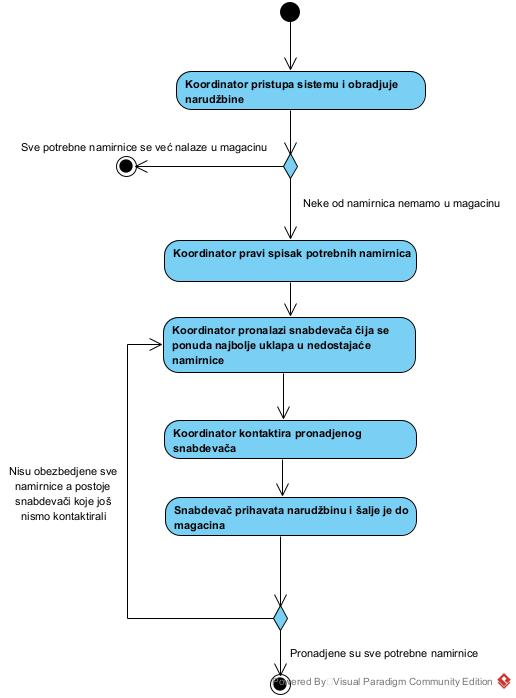
\includegraphics[width=\textwidth]{activity_diagram_order_placment_for_groceries.jpg}
\end{center}
    \caption{Dijagram aktivnosti - Naručivanje namirnica od snabdevača}
\label{fig:Activity_diagram_order_placment_for_groceries}
\end{figure}
